% 完整编译: xelatex -> bibtex -> xelatex -> xelatex
\documentclass[UTF8,AutoFakeBold=1,AutoFakeSlant,zihao=-4]{cucugthesis}

\usepackage{enumerate}


% 在这里填写你的论文题目
\newcommand{\thesisTitle}{如何使用{\LaTeX}生成本科毕业论文}  % 论文的中文名称
\newcommand{\thesisTitleEN}{Generation of an Undergraduate Thesis Using {\LaTeX}}  % 论文的英文名称

% 在这里填写你的相关信息
\newcommand{\yourDept}{计算机与网络空间安全学院}
\newcommand{\yourMajor}{计算机科学与技术}
\newcommand{\yourName}{刘逸珑}
\newcommand{\yourNameEN}{Y. Zhang}
\newcommand{\yourClass}{2017级计算机科学与技术}
\newcommand{\yourMentor}{周老师}
\newcommand{\studentID}{201720111222333}

\begin{document}
% 封面(自动生成)
\coverpage

% 中文摘要
\begin{abstract}
在准备毕业论文的过程中,学生们经常会被文本格式的设置与调整等问题所困扰。究其原因主要有以下两点:(1)使用Microsoft Word进行论文的编辑与排版,能够产生``得所见即所得''的效果,但是格式的设置通常非常繁琐,大家需要从准备毕业设计工作中分出很多时间与精力来投入其中。(2)一旦学院对本科毕业论文的格式有所调整,传达给学生时很难保证大家都能领会新的要求并完全执行到位。因此,我们准备了一个本科毕业设计的Latex模板,连同论文格式的类文件一同提供给大家。希望能够为大家在准备毕业论文的过程中减轻负担,能够生成排版质量精美的论文。 
\keywords{本科毕业论文;{\LaTeX}模板;排版}     % 中文关键词
\end{abstract}

% 英文摘要
\begin{abstractEN}
Here comes the English version of your abstract...
\keywordsEN{undergraduate thesis, {\LaTeX}, typesetting}       % 英文关键词
\end{abstractEN}

% 目录(自动生成)
\contentpage

% \section{绪论}
这个部分直接从开题报告上面抄下来的,还没改

\subsection{项目背景及意义}
TODO 重新引用,检查内容是否合适

今年来,由于一系列计算机网络安全事件的出现,操作系统领域的安全性逐渐被国家重视。
无论是2017年知名闭源操作系统windows中爆出的 永恒之蓝 病毒,还是近年来伊朗核试验基地遭遇“震网”病毒袭击时间,亦或是最近这段时间 linux 操作系统所面临的开源软件 xz 源供应链投毒事件,无不告诉我们操作系统领域安全性的重要性。
作为国民生产生活所不可或缺的一部分,一旦我们没有办法能保障操作系统的安全性,个人计算机尚且可能会被窃取隐私数据,大型的科研计算机亦或是国防科工设备一旦由于操作系统上的后门而遭到入侵,必然会导致巨大的损失。
因此,操作系统作为现代化行业的重要生产工具,其安全性,稳定性和可靠性必然需要得到保障。

而随着 rust 这种新型的,通过强制类型类型声明,所有权检查机制,生命周期检查器等一系列方式保障安全性的编程语言的出台,逐渐有使用此类编程语言进行操作系统设计实现的实验。如 (LANKES 等, 2019) 就在其论文中剃刀了
使用 rust 高级语言代替在 unikernel 中进行开发常用的 c 语言的设想。甚至在后来(LANKES 等, 2020) 尝试将其最初的 HermitCore 重新通过 Rust 语言进行了相关的实现 (Rusty Hermit),结果证明 Rust 语言实现版本与 C 语言实现版本之间
不存在性能差异。同时,由于 Rust 独特的标记不安全代码的设定,在操作系统中有且仅有 3.27% 的代码的安全性需要特殊注意。基于类似于 (BOOS 等,2020) 提出的 Theseus 操作系统,与 (KUENZER 等, 2021) 等提出的 Unikraft 微库操作系统实现理念的理解
,贾越凯博士实现了一种将组件化与库操作系统结合在一起的,基于 Rust 安全性保障的新型操作系统 ArceOS。

这种操作系统类似于较早年间外核(ExoKernel)的设计类似,由于其主要设计在嵌入式平台等专用平台上进行使用,而非基于某种通用的硬件设备或者 VMM 虚拟机的尝试,在实现层面上面临了许多硬件层面的适配问题。

本次毕业设计主要是想要通过在这种不同于传统操作系统架构,如宏内核或者微内核的类 LibOS,Unikernel 架构下操作系统中实现一些简单嵌入式设备常见驱动的过程,为今后的学习打下坚实的基础,也同时为我国现代化操作系统的发展实现添加我的一份力量。

% \subsection{国内外研究现状}

\subsubsection{Unikernel 国内外研究现状分析}

出于成本考量进一步加剧。在功能复杂的操作系统,比如说 Linux 操作系统上运行轻量级服务会由于通用操作系统所进行的必要抽象
支付大量的开销(ANDERSON 等)(MASSALIN 等, 1989)。因此,找到某种方法以细粒度的定制操作系统是存在必要的。也因此 (ENGLER 等) 通过
一种名为 Secure Bingdings 的机制,将 LibOS 与其他用户库绑定在一起,允许应用程序以更加具体到硬件的方式对于底层硬件进行调用,
释放其性能而不受操作系统层面抽象的局限。但是这种实现方法由于机制内部会导致额外的上下文切换,同样会带来不必要的成本。
[ PESSÉ S, XIA Y, QIU L, 2015. 计算机系统原理讲义[EB/OL]//计算机系统原理(课程讲义). (2015-07-21)[2023-12-06]. https://unitial.gitbooks.io/csp/content/index.html.]。
同时,从底层硬件设备驱动的角度上来讲,一般这些设备只会针对于部分通用操作系统进行适配,由操作系统层面完成这类支持是没有效率的。

不过,由于云服务商对于不同环境中一致性和可移植性的需求,类似于 docker 这种容器化技术逐渐出现,(MADHAVAPEDDY 等) 基于容器技术或者
虚拟机管理程序提供的底层一致性平台上,提出了 Unikernel 这种专用的,单地址空间的使用库操作系统理念构造的组件化操作系统
,这种构建方式解决了如 ExoKernel 等操作系统所面临的,在底层硬件上的兼容性问题 ,提供了一个小型的,安全的,快速的工作负载。
同时,由于该操作系统在实现类似于一般操作系统的进程管理等功能外不提供额外如 Shell 等功能,
降低了由于外界侵入所产生的危害与攻击面,在实现了更大程度上的安全保障的同时,也使系统能够更加紧凑
\footnote{相较于一般的BIND DNS的Linux VM 镜像达到462MB,
根据他们方法生成的Mirage设备生成的镜像大小只要183.5kB
(没有实现所有功能集,但是包含了queryperf测试套件的必要功能,且可用于自托管项目)]的高度专业化单一用途设备虚拟机。 }
,根据用户需求进行客制化。

(KUENZER 等, 2021) 在他们的研究中提出了一种名为 Unikraft 的新型微库操作系统,这种操作系统通过其特殊的编译,链接系统
提供了完全模块化的操作系统基元和一系列高性能 API 以方便用户对于操作系统进行定制。不同于前者基于高度定制 c 语言程序链接实现的思路,
(BOOS 等,2020) 的开发实践中通过其对 Rust 高等程序语言的编译编译工具链的利用实现了类似的效果,他们提出了一种名为 Theseus 的操作系统
这种操作系统通过减少一个组件为另一个组件保留的状态来重新设计和改进操作系统模块化,在尽可能的将保障内核安全的工作转嫁给 Rust 编译器
进行实现的基础上实现了对于核心操作系统组件的实时演化与故障恢复。不过,由于其代码特性,该操作系统实现的颗粒度相对更大,
不利于一般开发者参与进行开发。
贾越凯博士提出 ArceOS 的在其基础上粗放了对应核心组件的颗粒度,使得大部分的操作系统组件都可以以更加合乎一般操作系统开发者的开发
方式进行实现,在降低开发难度的同时,也实现了安全保障。


% (4)(PORTER 等) 在他们的研究中通过将广泛使用的单片操作系统(Windows 7)重构为一个功能丰富的库操作系统(Library OS),
% 由一个小型抽象集(线程,虚存,I/O流)连接 Library OS 和 Host OS实现了独立于底层内核组件。
% 在早期的 Library OS 支持者中认为,通过个性化定制每一个应用程序,可以实现OS的较好性能,
% 但是现在Library OS已经成为了现代虚拟机监视器的牺牲品。 作者在本文中通过将每个Library OS的特性(应用程序依赖的) 共享底层的 
% Host OS 资源,这样在操作中,只需要根据应用程序的API进行提取,这样相较于虚拟化整个OS会大大的降低开销。
% % \footnote{\href{source}{https://blog.csdn.net/qq_40119224/article/details/118754160}}

\subsection{研究目标}

1、研究的主要内容
本次研究主要分为以下几个目标,搭建嵌入式环境,编写指纹识别驱动以及网卡驱动实现。

2、研究的预期目标
能够在同一网段下实现或者更小的嵌入式开发板的相互通信,并且能够在Client端获取输入的指纹信息,将其加密后传输到Servers段进行解密,在解密之后Servers段传送解密成功信息给Client端,Client端通过显示屏显示对应信息或者通过指示灯表示打卡成功的信息。

3、研究的创新点
    尝试通过一种新颖的组件化操作系统对于一个简单应用场景进行重构。

\subsection{研究方法}

首先先简单完成电脑中有关于Rust等内容的开发环境配置,同时根据Nix生成一套可重构的开发环境框架,确保在后面的开发过程中整体开发过程是可复现的。
其次,深入了解现有的网卡驱动开发经验,并且了解其中所遇到的问题以及可能性的解决方案。在此基础上对于As608指纹识别模块驱动的现有实现进行了解,了解其中主要使用的数据结构等内容,以方便后面通过rust语言对于现有驱动进行重构。
然后,通过对于现有的指纹识别系统的分析,了解到目前常用的指纹识别框架。尝试了解no\_std情况下以及std情况下开发的差异。同时分析可能需要用到的库大概有多少是需要重新实现或者替换库的。
通过ArceOS现有的工作完成网络联网测试,实现几个简单的用户程序,首先确保能在多台华山派CV1811H甚至支持更少功能的嵌入式设备上运行简单发包程序并且联网成功。根据已有驱动尝试在ArceOS上进行测试等开发工作,最终将指纹识别驱动以及可能会用到的显示屏驱动,装载上进行整机测试。

引用图\ref{fig},表\ref{tab},公式\eqref{eq:0}
  % 第一章,在保存.tex文件时一定使用UTF-8编码。
% \section{系统设计}

\subsection{需求分析与模块选型}

\subsubsection{系统功能需求分析}

根据一般企事业单位对于考勤事务的管理规范,本指纹考勤系统需要实现以下几种功能,通过上位机对于下位机中指纹识别模块保存的指纹信息进行注册与删除,下位机基于前者提供的指纹数据实现基于光学识别的指纹打开签到功能。

\subsubsection{系统方案设计与选型}

根据上述系统功能需求,以树莓派4B所提供的 bcm2711 作为中央处理芯片,指纹考勤系统主要由电源供电模块,声音反馈模块,USB转TTL串口通信模块,网卡模块。
系统总体设计方案如图2.1所示。

% https://www.processon.com/v/65ec0156778cc21034664557
\begin{figure}[ht]
    \centering
    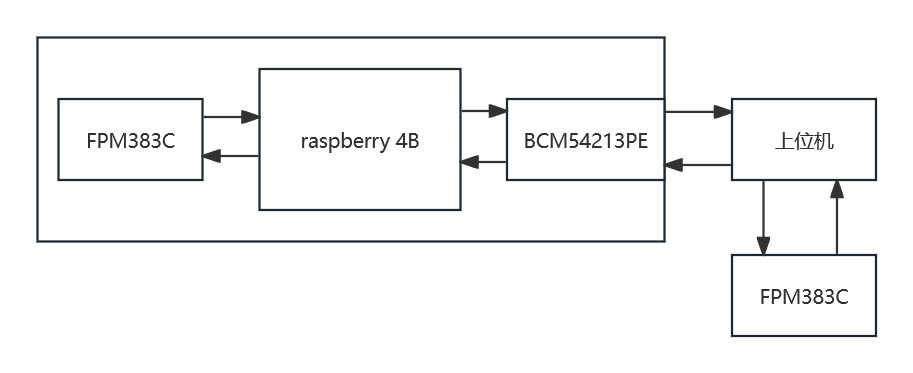
\includegraphics[width=\textwidth]{imgs/总体设计图.png}
    \caption{总体设计图}    \label{overall_design}
\end{figure}

\subsubsection{中央处理芯片选型}

树莓派4B使用的 bcm2711 是一种四核心64位ARM Cortex-A72架构CPU,主频高,能满足多种复杂计算需求以及满足大型程序运行需求。
树莓派4B还存在丰富而完善的接口,两个USb3.0接口,两个USB2.0接口,一个千兆网卡接口,一个HDMI接口,一个CSI接口和一个DSI接口,能够满足对于各种外设的连接需求。
树莓派4B还是树莓派第一个支持不通过 usb 直接访问网卡芯片实现网卡介入的开发板,这无形之中对于实现板载网卡驱动提供了很多帮助。

\subsubsection{指纹识别模块选型}

FPM383F识别指纹模块功耗低半导体面阵传感器是一款低功耗的光学指纹识别模块,支持对于60组光学指纹进行存储,其通过串口与中央处理器进行通信,在串口驱动方面,使用我开发的 arm\_gpio 库应当开发难度不难。

\subsubsection{通信模块选型}

    基于一般企事业单位对于考勤签到需求的需求,我计划提供多种不同的通信模块实现方便选用单位进行选择,
    其中传统基于 CH304 串口转 TTL 通信模块实现的简单串口通信主要适用于仅对于一两台设备进行支持的情况,
    而基于网卡模块间接通过网络方式拓展下位机数量的方式是主要计划实现的支持。
    针对于不同的预算管理需求,计划采用两种不同的方式实现网卡驱动,
    一种是基于 raspberry4B 板载 bcm54213PE 网卡芯片的驱动,
    另一种是基于 ENC28J60,一种基于 SPI 连接的外置 10BASE-T 以太网连接模块实现的。
    但是目前只实现了基于 BCM54213PE 网卡芯片驱动的支持。

\subsection{硬件设计}

    由于本实现相对来说比较轻量化,不太需要外部模块的支持,因此只是在面包板上完成了对应的实现,并没有画对应的板子。

    \begin{itemize}
        \item 信号回返模块:
            本模块主要实现的功能在基于树莓派电信号输出,实现简单的蜂鸣功能以提醒用户当前进行的打卡已经被正确识别。
            目前有两种实现的方法,一种是基于三极管实现的长延时信号灯,另外一种是基于无源蜂鸣器实现的。
        \item 指纹采集模块:
            本模块使用了现成的串口通信指纹识别模块予以完成。
        \item 网络通信模块:
            本模块主要使用了现有的树莓派板载 PHY 芯片 BCM54213PE 实现了对应的功能,同时
            还提供了串口替代的 USB 通信方法。
    \end{itemize}

\subsection{软件设计}

    由于本研究所采用的基础嵌入式应用程序所面对的的嵌入式应用场景相对较为单一,同时也是单应用程序单地址空间的。
    \footnote{虽然底层操作系统支持使用页表进行隔离,但是在应用层面上并没有使用到虚拟页表,只是在boot的时候使用了内核页表}
    因此整体软件设计相对较为简单,主要实现难度在驱动设计层面体现,具体内容与开发过程在第三章中进行呈现。
    在嵌入式应用层面只通过循环读取 UART 串口设备驱动反馈的数据,将其分析之后的结果通过由 ArceOS 包装底层以太网驱动实现的
    UDP 包经由 RJ-45 向上位机中运行的简单管理应用程序中发送。

    在上位机中通过简易的 python 客户端程序,对于嵌入式设备中传输的 UDP 包进行分析,实现基于 Sqlite 数据库的简单指纹信息 CRUD,打卡数据 CRUD,
    与一个基于命令行实现的打卡记录查询与导出应用程序。

    \begin{description}
        \item[指纹注册] 由上位机中自动完成指纹注册,通过上传命令,获取对应ID的指纹特征信息并以UDP包的形式下发到下位机中的指纹模块。
        
        指纹注册功能主要在上位机中完成,这主要是考量到在 HR 处实现人事登记等操作
        更加合乎一般企业的考勤流程。
        
        通过 0x0118 命令\ref{uart::auto-register},实现自动注册功能,该命令会自动完成采图、提取、拼接、保存等操作,
        在这个部分,通过对于回返包中 ID 以及注册进度的指示,在注册进度达到 0x64 时终止注册流程。

        \begin{table}[htbp]
            \resizebox{\textwidth}{!}{%
                \begin{tabular}{|l|l|l|l|l|l|l|l|}
                \hline
                \multicolumn{1}{|c|}{校验密码} & CMD类型 & CMD号 & 等待手指 & 按压次数 & ID\_H & ID\_L & 校验和  \\ \hline
                0x00 0x00 0x00 0x00        & 0x01  & 0x18 & 0x01 & 0x06 & 0xFF  & 0xFF  & 0xE2 \\ \hline
                \end{tabular}
            }
            \caption{自动注册命令用户层帧} \label{uart::auto-register}
        \end{table}

        在注册完成之后,通过上载命令\ref{uart::upload-info},向指纹模块获取特定 ID 号的指纹特征信息长度,
        然后再通过 \ref{uart::upload-data} 命令,从指纹模块获取对应分片的指纹特征信息。
        在将信息存储到数据库的同时,还通过 UDP 包的形式,将对应的数据发送到树莓派,树莓派再将对应指纹特征信息
        下载到树莓派对应的指纹模块上,由此完成了一次标准的指纹注册功能。

        \begin{table}[htbp]
            \resizebox{\textwidth}{!}{%
                \begin{tabular}{|l|l|l|l|l|l|}
                \hline
                \multicolumn{1}{|c|}{校验密码} & CMD类型 & CMD号 & ID\_H & ID\_L & 校验和  \\ \hline
                0x00 0x00 0x00 0x00        & 0x01  & 0x53 & 0x00  & 0x01  & 0xAB \\ \hline
                \end{tabular}
            } \caption{获取上传信息命令用户层帧} \label{uart::upload-info}
        \end{table}

        \begin{table}[htbp]
            \resizebox{\textwidth}{!}{%
            \begin{tabular}{|l|l|l|l|l|l|l|l|}
                \hline
                \multicolumn{1}{|c|}{校验密码} & CMD类型 & CMD号 & ID\_H & ID\_L & NUM\_H & NUM\_L & 校验和  \\ \hline
                0x00 0x00 0x00 0x00        & 0x01  & 0x51 & 0xFF  & 0xFF  & 0x00   & 0x00   & 0xAC \\ \hline
                \end{tabular}
            } \caption{获取指纹特征命令用户层帧} \label{uart::upload-data}
        \end{table}

        \item[指纹删除] Detailed explanation of functionality 2.
        \item[指纹考勤登记] Detailed explanation of functionality 3.
        \item[考勤记录读取] Detailed explanation of functionality 3.
    \end{description}
      

  % 第二章
% \section{系统开发流程}

    按照现有嵌入式企业的嵌入式软件开发流程,开发一个嵌入式系统主要分为以下几个步骤。

\subsection{用户需求分析}

    根据现有的各种企事业单位对于考勤打卡的需求,在考勤系统中最核心的功能特性是特征性识别和日志记录功能。
    
    因此,在总体设计上本研究计划采用最简单的由指纹识别模块获取输入,经过 MCU 中简单处理再转发给
    linux 下的控制主机的设计。

\subsection{嵌入式开发环境的搭建与说明}

    由于嵌入式开发所基于的 MCU 一般性能相当有限,就算是采用一般 linux 操作系统进行本机编译,其占用时间也会相对比较长,同时,也无法应对一些占用系统内存资源较大的编译场景。
    因此,在嵌入式开发中,一般通过交叉编译的方式实现在 x86\_64-linux 平台或其他通用操作系统架构平台上实现对于目标平台代码的编译以更好的利用硬件资源。

    在本文的实现过程中基于 \href{https://nixos.org/}{Nix} 管理 x86\_64-linux 平台实现了对 aarch64-unknown-linux 目标平台的编译,
    其中主要的编译工具链的部分直接采用原有 \href{https://github.com/rcore-os/arceos}{ArceOS} 操作系统实现的 Rust 语言交叉编译以及镜像处理步骤
    ,将 Cargo 包管理工具直接生成的裸机 elf 文件通过 rust-objcopy 去除其中如调试信息等无关内容成为一个纯粹的二进制文件。 
  
    通常,树莓派启动流程开始于 Soc ROM 区中的 bootloader, 他负责挂在位于 SD 卡上的 FAT32 分区,并加载第二阶段的 bootcode.bin 文件。但是在本次采用的树莓派4B (bcm2711) 
    相对于前代有不少的硬件更新,其中中对应初始化,启用 GPU fireware 加载 start.elf 的 bootloader 代码都被实现在 EEPROM 中。
    在运行 start4.elf 文件时,其会对 sd 卡中的 config.txt 文件进行解析,完成对应如串口传输频率,是否启用 JTAG 调试等配置,
    还会将其中声明的镜像文件加载到内核默认加载地址地址,使 CPU 由 stand-by 状态开始执行内核初始化代码。

    在我开发的过程中参照 \href{https://github.com/rust-embedded/rust-raspberrypi-OS-tutorials}{rust-raspberrypi-OS-tutorials} 
    的串口传输工具完成了串口传输的配置。其中通过实现一个最小配置内核,实现了初始化对应端口(PIN 14,15)的替代方法声明以启动对应端口的传输声明。
    同时通过 CH340 USB 转 TTL 串口传输模块发送开始传输信号给开发机中 Ruby 运行的应用程序,应用程序将内核镜像文件通过串口传输到树莓派4B内存中以完成镜像加载。
    最终最小配置内核将控权转交给内核镜像文件,来配置基础的,基于串口传输的二进制镜像文件传输配置。

    同时,基于开发环境一贯的可重构性,易重构性,同步性的需求的考量,我选用了 \href{https://nixos.org/}{Nix} flakes 对于项目整体依赖进行管理。
    就目前来看,除了对于使用到其他项目中的 docker 的部分,由于在 Non-NixOS 中,Nix 无法介入 systemctl 的管理而存在一定的不一致情况以及由于 WSL 对于串口设备连接的限制
    \footnote{在WSL中连接串口设备的时候,需要额外安装 usbipd},其他的部分表现良好,均能很好的在 WSL, NixOS, Debian 等常用开发系统中构建一致,可用的开发环境。

    具体在实现过程中,我通过 flakes.inputs 固定了后面引用的 Nixpkgs, rust-overlays 库。
    同时,使用 overlays 在原先 nixpkgs 上掩盖了我自己的派生以保证开发环境构建的一致性。
    在附录代码段\ref{nix-flake} 第 23-32 行实现了对于 rust nightly toolchain 的固定,
    在 33-39 行实现了对于 nixpkgs 特定版本 qemu 的选择,在 40-51 行实现了对于联网获取的编译工具链的固定,61-74行实现了必要依赖软件的声明。
    同时,为了保证引入的工具链能完整的运行,
    我根据 \href{https://github.com/nixos/nixpkgs}{nixpkgs} 中提出的 issue,对于部分存在的问题进行了修复(见 77-86 行)。

\subsection{ArceOS 操作系统现有 cvitek 网卡驱动实现分析}

    下图\ref{fig::cvitek}左侧的部分是 ArceOS 操作系统的整体布局,右侧是现有\href{https://github.com/yuoo655/arceos_net/tree/hsp}{cvitek 物理网卡驱动} 的逐层调用情况。

    该 cvitek 物理网卡驱动主要作用在华山派,荔枝派等主机上。但与我们采用的树莓派4B中由 Soc 中集成 MAC 实现不一样,他们采用的这款设备提供了一个额外的以太网 MAC 控制器的 IP 核DWMAC 来完成 MAC 层的实现。

        
    \begin{figure}[ht]
        \centering
        \caption{cvitek 驱动调用栈}    \label{fig::cvitek}
        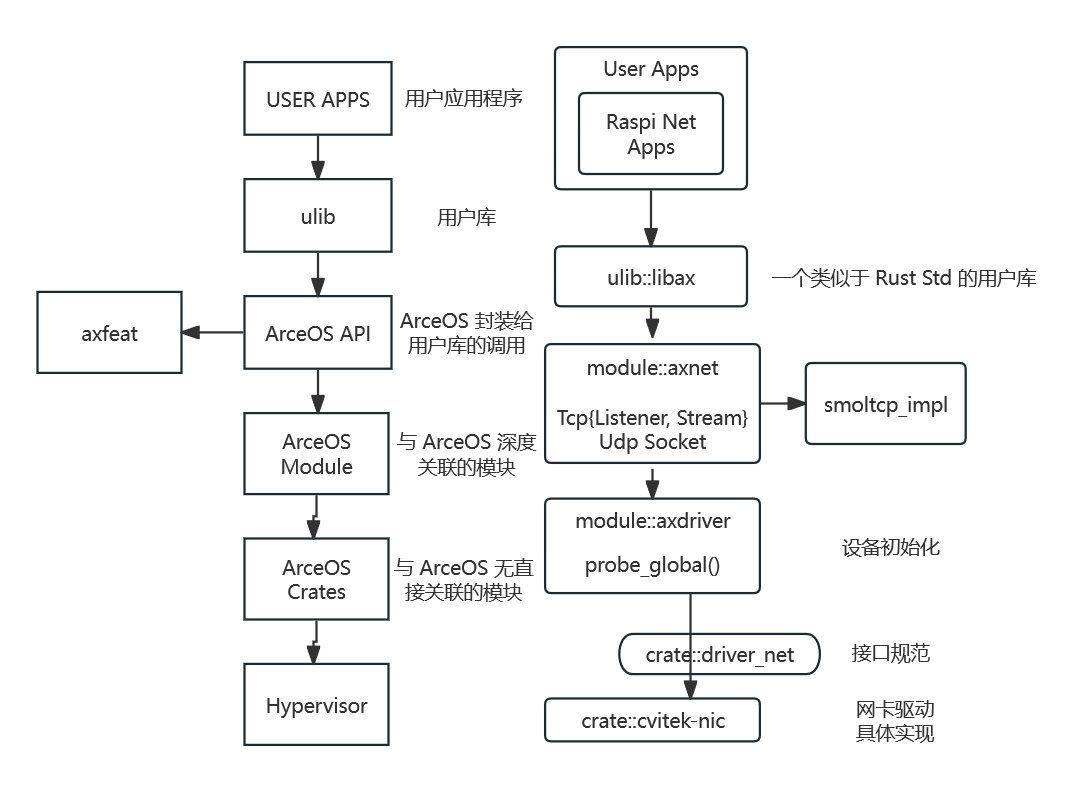
\includegraphics[scale=0.4]{imgs/cvitek.jpg}
    \end{figure}

    在整套实现中,ulib::libax 通过调用 module::axnet 所实现的底层方法(如TcpSocket,UdpSocket等)实现了用于 TCP/UDP 通信的通信源语。
    在 module::axnet 中这个部分的实现是针对于 
    \href{https://github.com/smoltcp-rs/smoltcp}{smoltcp} 这个 tcp/ip 协议栈进行了针对性的改造(非标准库环境等改造)而完成的。
    如果在编译的时候添加了对应的 features, ArceOS 会自动根据 module::axdriver::build.rs 文件中所进行的声明,
    将一个带有不同设备名称的 feature 加入默认 feature list 中,以方便实现基于设备组(phy, net, block, display) 实现的自动驱动加载。
    在完成 build.rs 编译脚本中的检查等操作之后,Cargo 在对于 axdriver 进行编译的时候,
    就会识别到当前编译携带了 cvitekphy/nic feature 从而根据 \#[cfg(feature = "cvitekphy")] 启用 cvitek\_traits.rs 的编译。
    cvitek\_traits.rs 文件将 ArceOS 上层 module 所提供给下层 crates 的方法支持(如dma\_alloc\_pages,delay等)
    通过 traits 的默认实现传递给下方的 crates 进行使用以实现 crates 层逆向调用 modules 层方法的效果。
    \footnote{在cvitek\_traits.rs 文件中 CvitekPhyTraits 声明并实现于 CvitekPhyTraitsImpl }。
    同时,在 module::axnet::driver.rs 中基于 cfg\_if 库的条件编译语句也实现了将 cvitek 网卡驱动转换成为 AxNetDevice 
    并实现了 Driver traits 下属的 probe\_global 方法的效果。
    最后在 module::axdriver 中 for\_each\_driver 宏的帮助下,ArceOS 将各个加载的网卡驱动转换成为 
    Driver 并运行(probe\_global)初始化,并将其添加到 AllDevices 下属的结构体中。

    而根据 ArceOS 的规定,cvitek 以太网卡驱动的实际实现实际上被封装在各自的 crates 中。在 crates::driver\_net 包规定了一系列网络设备、
    所必须要实现的 traits(如 transmit, receive)等方法。
    新的网络驱动会使用其内部方法实现这些对应的 traits,将这些方法包装成为 ArceOS 的调用方法。

\subsection{BCM54213PE 以太网卡驱动分析与实现}

    根据前文的分析,如果想要实现在 TRANSPORT 层或者 NETWORK 层实现树莓派和主机之间的通信效果,主要需要实现以太网 OSI 七层模型中的 DATA\_LINK 与 PHYDIVSL 层之间的通信,
    由下图\ref{fig::dataLink}可知,主要需要实现的部分在于使 Soc 上的 MAC 实现能通过 GMII, RGMII,Serial-GMII 等接口标准与 PHY 芯片进行联通,进而调用 PHY 芯片上对于以太网传输介质上光,电等信号进行解析的方法。
        
    \begin{figure}[ht]
        \centering
        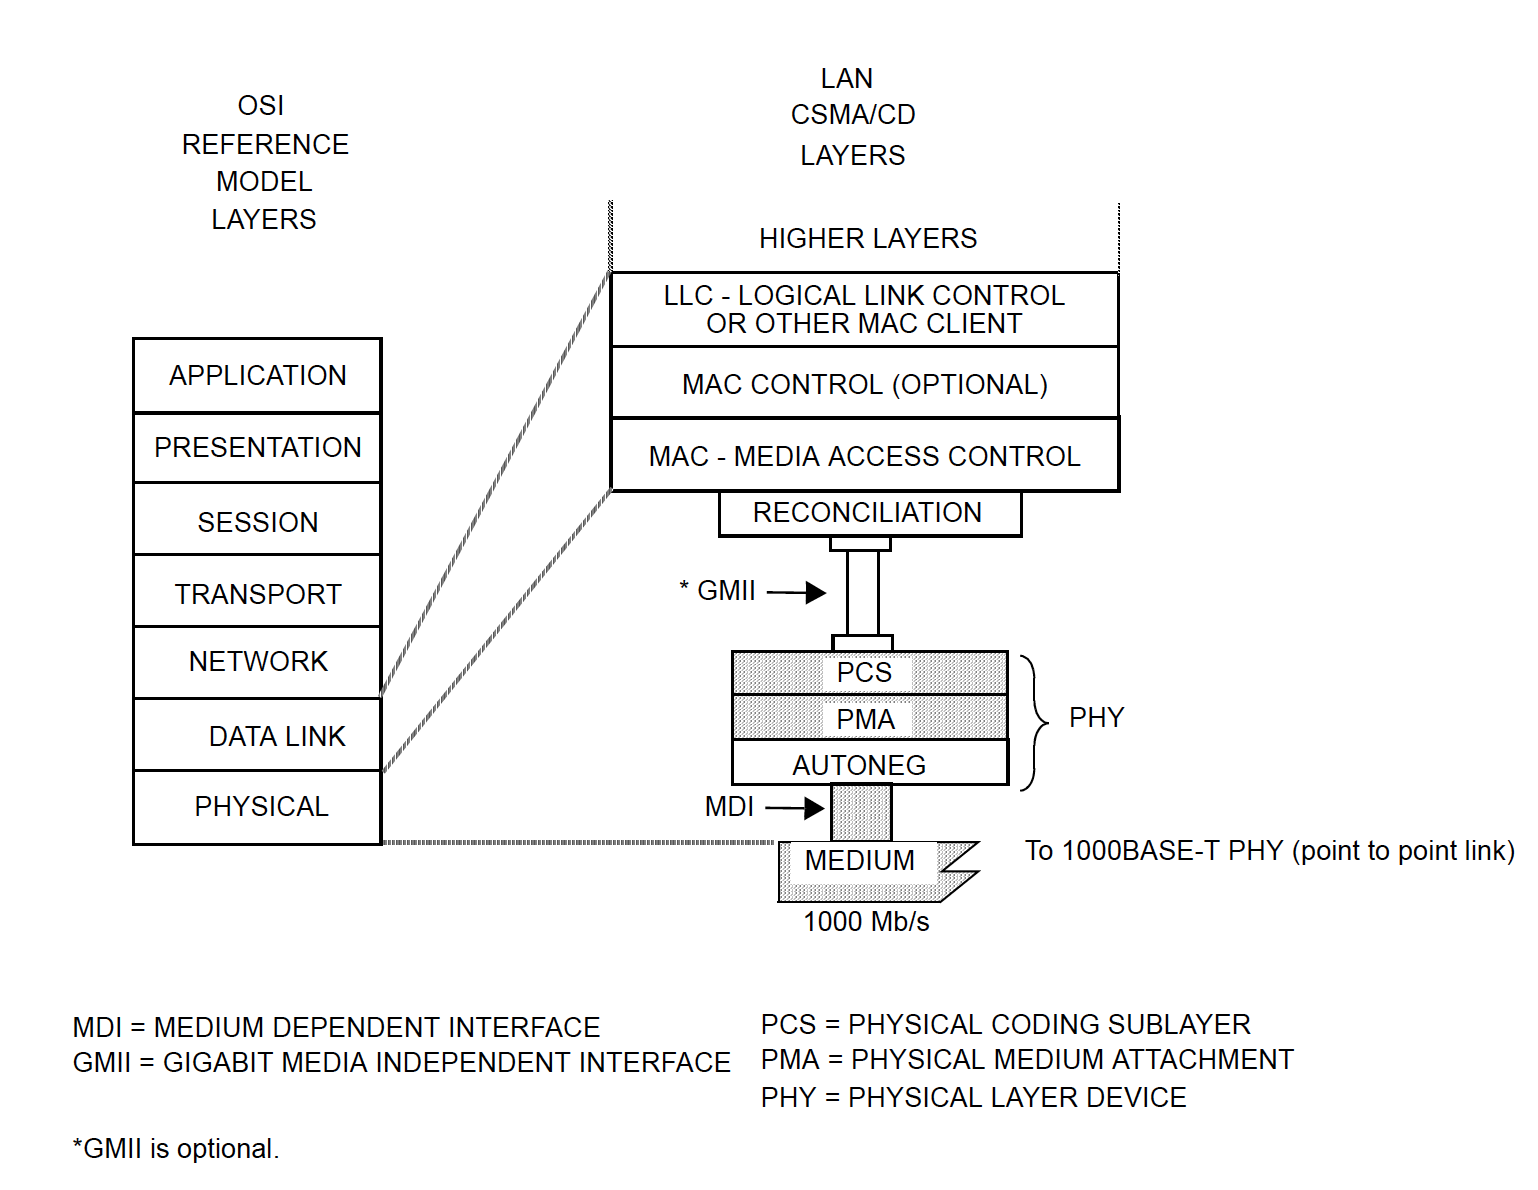
\includegraphics[scale=0.4]{imgs/data_link_layers.jpg}
        \caption{IEEE 802.8 数据链路层}    \label{fig::dataLink}
    \end{figure}

    基于 树莓派 4B Soc bcm2711 芯片手册,其板载 PHY 芯片 BCM54213PE 数据表以及 IEEE 802.3 协议手册可以了解到,目前 Soc 和 PHY 之间是存在直连的 RGMII 通信接口的。
    在 RGMII 通信接口中由 GTK\_CLK, RX\_CLK 实现双向时钟同步,TXD[0:3], RXD[0:3] 实现数据传输,TX\_CTL,RX\_CTL 实现数据传输控制,MDIO 和 MDC 实现 MAC 与 物理层的控制和状态关系的设置。
    \footnote{虽然在bcm2711数据手册GPIO替代函数表中有提到提供了 RGMII\_MDIO 与 RGMII\_MDC Pins,但是没有找到任何公开资料描述这个部分与底层之间是如何联系起来的}

    % TODO: 其中 GPIO 中也提供了一组 MDIO MDC 有点没太明白这段是为什么添加到这个地方?

    % \subsubsection{源码分析}


    \begin{minipage}[t]{0.42\linewidth}
    \begin{lstlisting}[columns=fullflexible]
       +
0x0    | IOBASE
+------|-----------------------------+
0x2000 | GENET_RX_OFF
       | [DMA_DESC_SIZE;TOTAL_DESCS]
0x2C00 | GENET_RDMA_REG_OFF
       | [DMA_RING_SIZE;DEFAULT_Q]
0x3000 | RDMA_RING_REG_BASE
       | [DMA_RING_SIZE]
0x3040 | RDMA_REG_BASE
       | dma_reg
+------|-----------------------------+
0x4000 | GENET_TX_OFF
       | As above ...
        \end{lstlisting}
        \captionof{figure}{BCM54213PE内存分配示意图\label{fig::uboot-genet-struct}}
    \end{minipage}
    \quad
    \begin{minipage}[t]{0.5\linewidth}
        \vspace{2em}
        \setlength{\parindent}{1em}
        根据对于 uboot 源码所进行的分析,在以太网 PHY 芯片中维持了如图\ref{fig::uboot-genet-struct}所示的数据结构。
        其中,IOBASE 为 BCM54213PE 芯片寄存器通过 MMIO 映射到树莓派内存中对应的地址起始地址。

        在树莓派网卡中,0x2000-0x4000的地址主要分配给与Rx相关的结构体。0x4000-0x6000的地址分配给TX相关的结构体。
        以 0x2000 GENET\_RX\_OFF 开头,到 GENET\_RDMA\_REG\_OFF 为止的一段地址中保存了 256 个 DMA 描述符结构。
    \end{minipage}

    以 0x3000 GENET\_RDMA\_REG\_OFF 开头,到 RDMA\_RING\_REG\_BASE 为止的这一段地址中保存了 BCM54213PE 
    所支持的 16 个不同优先级别的接受环(方便 DMA 实现基于不同优先级的接受),
    还在 RDMA\_RING\_REG\_BASE 与 RDMA\_RING\_REG \_BASE 之间保存了一个默认的接受环。

    也就是说在 BCM54213PE 的硬件实现中提供了对于 16 个优先级队列,以及一个默认队列的支持。不过根据源代码,
    实际上不管是树莓派官方的 linux 内核或者 uboot 下的以太网驱动都没有全部使用这些队列。
    在树莓派中,将 256 个 DMA 描述符分配给五个队列,其中前四个队列分别占有 32 个描述符,第五个,也就是默认队列
    占有剩余的 128 个描述符。而在 uboot 中的实现考虑到了其需求,对于原先的设计进行了删减,
    直接将 256 个 DMA 描述符全部分给了默认队列(并没有使用优先级队列)。
    
    \begin{adjustwidth}{0cm}{} % NOTE: 消除全局段首锁紧带来的影响
    \begin{minipage}[b]{0.5\linewidth}
        \setlength{\parindent}{2em} % 段首缩进
        在 BCM54213PE DMA 模块中以太网模块初始化的过程中,会逐个将使用的 Rings 环进行初始化,
        每一个抽象意味上的环都是由 start\_addr 到 end\_addr 中的一段连续的 DMA 描述符组合而成的。
        每一个DMA描述符指向一段特定长度的内存空间,这也就是后文所提到的缓冲区的概念(见附录代码段\ref{code::InitRxRings})。

    \end{minipage}
    \hfill
    \begin{minipage}[b]{0.45\linewidth}
        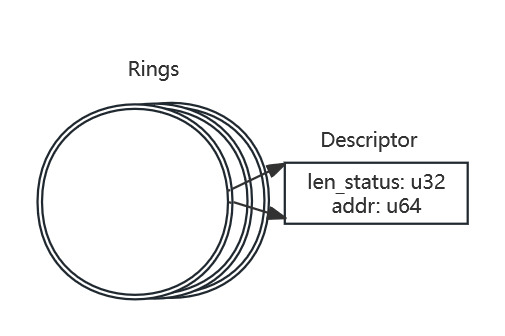
\includegraphics[scale=0.6]{./imgs/Rings_and_Descs.jpg}        
        \captionof{figure}{DMA 描述符与环} \label{pict:DmaDescAndLoop}
    \end{minipage}
    \end{adjustwidth}
    
    在具体实现层面其实没有什么特殊于前者的,由于 BCM54213PE 的相关寄存器手册不对外公布,大部分的寄存器操作都是
    从 u-boot 或者 树莓派 linux 中进行的参考,只不过是根据 tock-registers 有界寄存器规约,
    将原本 u-boot 中存在的大量由宏或者裸地址进行声明的地址位置转变成为了 rust 语言下的定义,并且利用其边界检查等功能,进一步的
    保证了寄存器的操作的安全性,同时也提供了更加符合人体工学的寄存器操作(见附录代码段\ref{code::tock_register})。

    \begin{figure}[ht]
        \centering
        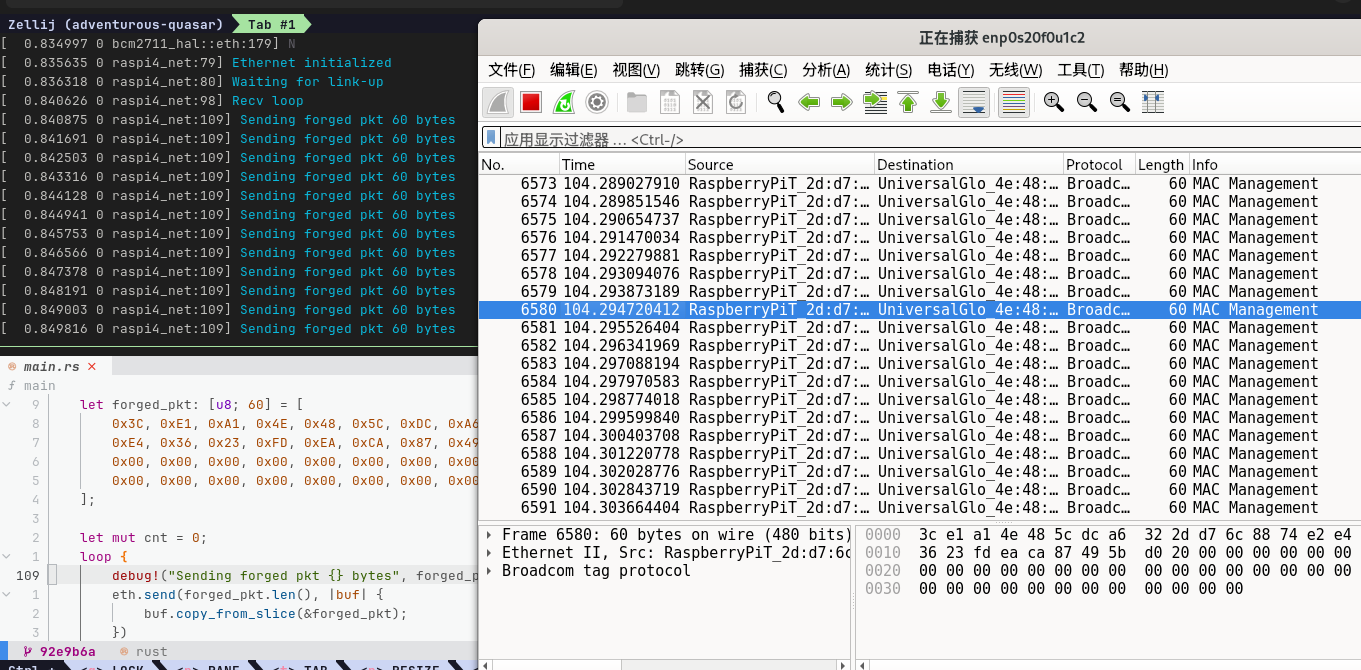
\includegraphics[scale=0.3]{./imgs/以太网帧通信正常.jpg}
        \caption{以太网帧通信正常}    \label{fig::树莓派通信正常}
    \end{figure}

    在进行了大量的适配以及检查之后,如上图\ref{fig::树莓派通信正常}所示在树莓派层面上成功完成了收发以太网数据帧的操作。
            
    完成基础的以太网帧的收发之后,接下来的操作就是参照现有 Cvitek DWMAC 驱动逐步转写 BCM54213PE 以太网驱动,在实现以太网帧收发后
    再利用现有 ArceOS 实现的以太网协议栈使用户程序可以直接使用 axstd 中 Udp 支持调用底层相关服务。
    \footnote{根据实现要求,在树莓派下位机上实现基于以太网帧直接发送对应数据给指定的物理地址是不利于
    本设计通过网络进行拓展的(对于单一企业而言,存在多个打卡机属于正常现象),因此必须要能实现基于 Udp 的打卡信息发送功能}
    ,最终实现一系列的基于 UdpSocket 的包传输。

    \noindent
    \begin{minipage}[t]{0.40\linewidth}
            \vspace{0pt}
            \centering
            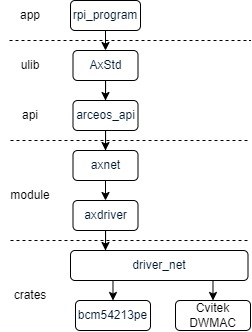
\includegraphics[scale=0.6]{./imgs/ArceOS_网络调用.jpg}
            \captionof{figure}{ArceOS 网络调用}    \label{fig::ArceOS网络调用}
        \end{minipage}           
        \quad
        \begin{minipage}[t]{0.55\linewidth}
            \vspace{0pt}
            \setlength{\parindent}{1em}

            我根据本次毕业设计要求设计的应用程序
            利用一个名为 AxStd 的类 Rust Std 库间接调用由 arceos\_api 提供的接口。
            这个设计巧妙的允许了应用程序同时在两种不同的情况
            \footnote{基于标准 Std 库与在嵌入式板子上基于自带库}
            下进行调试,此外,接口的实现可以通过功能标签(feature flags)进行切换,以方便切换底层实现以适应不同的需求。

            arceo\_api 接口通过对于底层 axnet 提供的各个不同方法的调用来实现具体的内容,这个模块内部
            利用 smoltcp 这个现成的以太网调用堆栈,完成以太网协议中网络层、会话层的实现。他在底层依赖于
            axdriver 内部完成的驱动加载,与 driver\_net 中所应以的 NetDriverOps traits。           

        \end{minipage}

    % TODO: 考虑添加图片说明这个过程

    % TODO: 后面看是用我自己的驱动还是直接用现成的

    \subsection{FPM383F 指纹识别模块串口通信单元分析与实现}

    UART(Universal Asynchronous Receiver/Transmitter,通用异步收发传输器)也常被称为串口。
    UART 总线是在开发中使用频率最高的数据总线,其最大的特点就是在其上进行传输的时候仅需要三根信号线(TX,RX,GND)
    就可以实现基本的信号传输功能而不需要常见同步传输所需要的时钟线。

    在这种异步收发传输器上,由于没有如同同步通信时所享有的时钟信号,需要以一种特殊的方式对于一个二进制信号的起始与终止进行规范,
    以方便进行读取的时候能够将信号线上进行传输的高低电平正确的转换成为二进制信号,UART 中要求通信双方设置波特率为相同值,
    两边模块基于波特率对于信号线上的电平进行采样,就比如说当前指纹模块与树莓派主控模块之间采用的是 57600Bps,
    就相当于在信号线上进行通信的时候,每个信号占据 1/57600 s。

    在信号线上没有进行传输的时候,信号线上保持高电平。在传输开始时,发送端会特地给一个低电平作为传输开始标记
    接受端收到了这个信号之后根据前面规定的每隔 (1/波特率) 秒对于信号线电平进行采样,将八个电平信号转换成为实际的字节数据。

    \begin{figure}[ht]
        \centering
        
\includegraphics[scale=0.4]{imgs/UART跳变图.png}
        \caption{UART 跳变图}    \label{fig::uart}
    \end{figure}

    FPM383F 通信协议要求在串口层面使用小端序,十位帧格式(1位起始位,1位停止位,8位数据位),默认采用 57600Bps进行数据传输。
    \cite{noauthor_fpm383c_nodate}

    根据 FPM383F 通信协议的规定,串口层面传输的字节数据,在链路层面实际上以类似于下文中的数据结构\ref{FPM383F::UARTdataFrame}进行存在,
    在进行发送的时候逐个字节的进行传输。\cite{fpm383c-modular-communication-protocol}
    从软件层面上讲,无论是发送还是由串口接收数据,均只需要对于对应 UART 的 DR 寄存器进行逐个字节读取或写入即可,具体内容被实现在硬件层面。
    
    \begin{table}[H]
        \centering
        \caption{UART 数据帧格式表} \label{FPM383F::UARTdataFrame}
        \begin{tabular}{lllll}
        \hline
        格式        & 帧头 & 应用层长度 & 帧头校验和 & 应用层数据 \\ \hline
        长度(bytes) & 8  & 2     & 1     & 7+N   \\ \hline
        \end{tabular}
    \end{table}
    
    根据 FPM383F 通信协议的设定,应用层面其实由两种类型的命令构成。一种是主机向从机发送的请求,如图 \ref{FPM383F::UARTUserRequest}
    所示,另一种是从机(FPM383F)响应主机的请求,向主机发送响应,如图 \ref{FPM383F::UARTUserResponse}

    \begin{table}[H]
        \centering
        \caption{UART 请求格式表} \label{FPM383F::UARTUserRequest}
        \begin{tabular}{lllll}
        \hline
        \multicolumn{1}{c}{格式} & 校验密码 & 命令 & 数据内容        & 校验和 \\ \hline
        长度(Byte)                 & 4    & 2  & N(0$\sim$n) & 1   \\ \hline
        \end{tabular}
    \end{table}

    \begin{table}[H]
        \centering
        \caption{UART 响应格式表} \label{FPM383F::UARTUserResponse}
        \begin{tabular}{llllll}
        \hline
        \multicolumn{1}{c}{格式} & 校验密码 & 命令 & 错误码 & 数据内容        & 校验和 \\ \hline
        长度(Byte)                 & 4    & 2  & 4   & N(0$\sim$n) & 1   \\ \hline
        \end{tabular}
    \end{table}

    我这里采用我实现过程中相对比较复杂的一个部分,对于主从机响应的整个过程进行说明,如图\ref{FPM383F::DownloadFingerPrintInfo}所示。
    在我们从指纹模块获取对应指纹信息并且上传到上位机的时候,我们需要先使用0x53命令,向串口模块请求上传对应 ID 的指纹信息,
    指纹模块在没有出现错误的情况下会反馈特征长度,同时错误码置为0。
    获取到该ID对应的整体特征长度之后,我们就可以通过循环命令,逐帧
    \footnote{根据通信手册,在同一帧下用户层最多只能添加128位的数据(在此处特指用于传输特征信号的信息位),因此需要逐帧进行发送}
    请求指纹模块上传该部分的指纹特征信息,最终在上位机将上述全部指纹特征信息整合到一起。

    \begin{figure}[H]
        \centering
        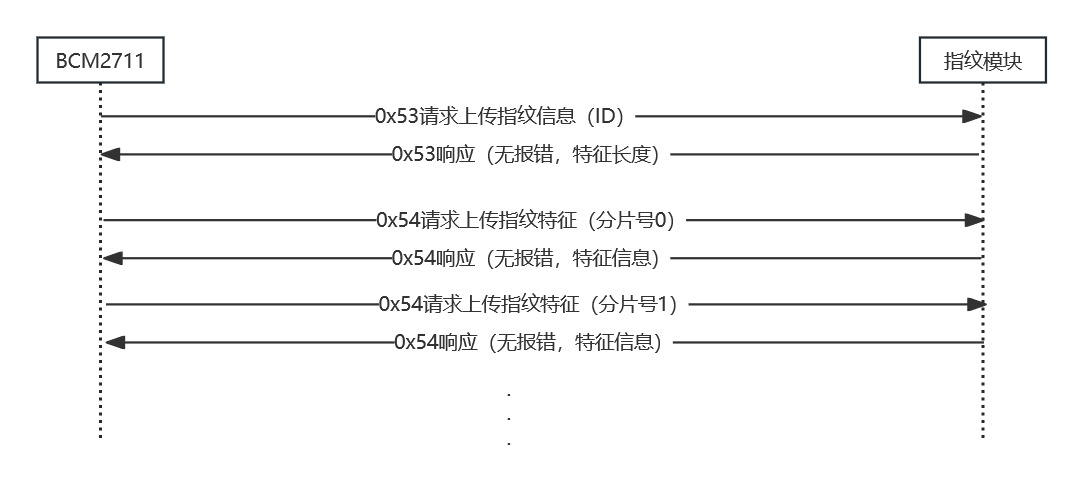
\includegraphics[scale=0.4]{./imgs/指纹信息下载.jpg}
        \caption{指纹信息下载}    \label{FPM383F::DownloadFingerPrintInfo}
    \end{figure}    

    在实现上,树莓派提供了一系列与 UART 相关的寄存器,如 UART0, UART1(mini), 
    UART2-5等,考虑到目前 GPIO 口的占用情况,我选用了 GPIO4,5 所对应的串口
    UART3 来完成串口信息交换。

    我参照 2020 年 jonlamb-gh rpi4-rust-workspace 仓库\cite{rpi4-rust-workspace}
    提供的基于树莓派 UART 的串口树莓派初始化方案,进行了大量的适应性修改,在原先仅实现了串口收发包的基础上
    实现了对于 FPM383F 通信协议的适配,实现了解析,生成等功能。同时,由于根据上位机中实现指纹注册功能的设计,
    我同样使用 python 语言在上位机中实现了对应的功能
    \footnote{没有找到任何基于py语言的实现,唯一一个\href{https://github.com/deerbleats/micropython-HLK-FPM383C}{micropython-HLK-FPM383C}, 是在嵌入式设备上完成的处理工作}。

    具体算法抽象如下:

    \begin{algorithm}[H]
    \caption{以太网帧解析算法}
    \label{algorithm::UART}
    \begin{algorithmic}[1]
    \renewcommand{\algorithmicrequire}{\textbf{Input:}}
    \renewcommand{\algorithmicensure}{\textbf{Output:}}
    % \newcommand{\Desc}[2]{\State \makebox[4em][l]{#1}#2}
    % \Desc{Input: }{matrix of measurements}
    \Require ser: 串口对象
    \Ensure (length: int, userLayerData: List[int]) 
    \Function{parse}{$ser$} 
        \State $frame\_head \gets [0xF1, 0x1F, 0xE2, 0x2E, 0xB6, 0x6B, 0xA8, 0x8A]$ \Comment{帧头固定}
        \State $frame\_data \gets$ array of size 256 filled with 0 \Comment{考虑到全局分配,暂时采用数组}
        \State $len \gets 0$
        \State $cnt \gets 7$ \Comment{帧头的最后一位为7}
        \While{true}
            \State $data \gets$ read one byte from serial port $ser$ \Comment{逐字节读数据}
            \If{$frame\_data[0:8] \neq frame\_head[:])$}
                \State $frame\_data[0:8] \gets frame\_data[1:9]$
                \State $frame\_data[8] \gets 0$ \Comment{清理残余}
                \State $frame\_data[7] \gets data$
            \EndIf
            \If{$frame\_data[0:8] == frame\_head[:]$}
                \State $frame\_data[cnt] \gets data$
                \If{$cnt > 11$}
                    \State $len \gets$ convert bytes to integer($frame\_data[8:10]$)
                \EndIf
                \State $cnt \gets cnt + 1$
            \EndIf
            \If{$len \neq 0$ and $(cnt - 11) == len$} \Comment{确保当前帧的全部数据均已被收集}
                \State \Return $(len, frame\_data[11:cnt-1])$ 
            \EndIf
        \EndWhile
    \EndFunction
    \end{algorithmic}
    \end{algorithm}
    
    考虑到实现的便捷程度,我并没有在下位机中实现对应帧的和校验,只是采用了简单的
    帧头循环方式,实现了对于串扰数据等因素导致的乱码使帧头校验不通过的情况进行了预防
    \footnote{但是这样就会出现一个问题,当某个字节收到影响没有被正确识别就会导致程序卡死}。
  % 第三章
% \section{设计结果论述与不足思考}

    指纹考勤系统以树莓派4B(BCM2711)为核心,包括以下组件:
    指纹传感器HLK-FPM383C、
    基于树莓派板载BCM54213PE PHY芯片的通信模块,
    以及由上位机提供的数据存储,日志记录的部分。\\

    \noindent 全文主要完成了以下六个方面的工作:

    \begin{itemize}
        \item 完成了指纹考勤系统整体设计,对于一个最简易的单片机指纹考勤系统进行了需求分析。
        \item 完成了指纹考勤系统硬件电路设计。主要包括主控模块与信号回返模块,串口输入模块之间的硬件电路设计。
        \item 在组件化操作系统 ArceOS 上仿照树莓派官方 linux 内核中驱动相关实现,实现并整合了一个能运行的以太网驱动,
            该驱动实现了以太网物理层与数据链路层之间的通信,
            嵌入式裸机应用程序可以深度集成到ArceOS中,调用由 ArceOS 实现的 Tcp/Udp 以太网协议栈以在应用层面调用 UdpSocket 所提供的服务编译成一个完整的单一用途裸机应用程序。
            通过这个以太网驱动,可以实现下位机与上位机之间的以太网帧通信\ref{fig::树莓派通信正常}。
        \item 将上述以太网驱动与 ArceOS 中提供上层网络包装的 axnet module\footnote{基于smlotcp的实现} 进行结合,
            实现了基于 UdpSocket 的发包功能。
        \item 在组件化操作系统 ArceOS 中,基于自建 UART 串口驱动与FPM383模组通信协议\cite{noauthor_fpm383c_nodate},
            实现了 ArceOS 的指纹模块,能基于串口信号传输,实现简单的如LED亮灯,要求FPM383C模块进行指纹匹配,
            对于收到的指纹匹配结果进行分析等功能。
        \item 根据上述指纹考勤系统设计需求,实现了一个基于 ArceOS 改写标准库的裸机应用程序。
    \end{itemize}

    \noindent 实现的不足之处:

    \begin{itemize}
        \item 参照树莓派 linux 内核中以太网卡实现的部分操作还没有调通,从 BCM54213PE PHY 芯片所返回的状态检查一直
        显示当前链路状态未建立,查阅了全部可能有关的状态寄存器,仍然无法明确具体这种情况是由什么原因导致的。
        幸运的是,在深入研究时我发现了一个名为 rpi4-rust-workspace 的代码仓库 \cite{rpi4-rust-workspace},
        在这个最后更新于 20 年的仓库中提供了一个相较于我实现更为完善的以太网卡驱动,只不过由于仓库维护者太久没有进行维护,
        在仓库中所引用的很多 rust 语言的方法没有办法在 ArceOS 所支持的 rust 工具链中正常运行。
        同时,仓库中也存在着很多由于维护者直接将 rpi3 版本中寄存器复制到 rpi4 版本的过程中没有详细检查寄存器等调用是否一致所导致的问题,
        比如说在 UART 驱动实现所牵涉到的 GPIO 部分\footnote{根据 FPM383C 模块说明,必须要在Rx设定上拉电阻},维护者直接将在
        rpi3(bcm2835) 使用的 GPIO Pull-up/down Register 也就是 GPPUD 寄存器等寄存器规约复制到了 rpi4(bcm2711)
        中\cite{raspberry-pi-bcm2835}。但是,树莓派 4 中采用了另外的一组寄存器 GPIO\_PUP\_PDN\_CNTRL\_REG0 来控制上拉下拉电阻
        \cite{raspberry-pi-bcm2711},二者类型不同,起始地址也不同。
        亦或是由于作者实现串口驱动的目的在于通过串口反馈简单字符串,并没有考虑到在大信息通量下的数据获取问题,因此没有启用 FIFO 等。
        \item 由于时间因素的影响,并没有如同前面设计的那样,实现了多种不同的上位机,下位机通讯机制,只完成了基于 BCM54213PE 板载
        PHY 芯片的网络通信机制实现。
        \item 在实现树莓派经由 BCM54213PE PHY 芯片与上位机进行通信的时候,由于时间因素的影响
        \footnote{就目前来看可能还需要 4 天以上的工作量},
        未能详细的对于 ArceOS 内部实现以太网协议栈的部分进行详细分析,因此在树莓派中接受网络包的时候仍存在一定问题,
        在实现指纹注册并下发的工况中
        \footnote{上位机中 python 后端程序调用串口,从上位机从属指纹识别模块获取指纹特征信息,并将对应指纹特征信息下发到树莓派从属指纹识别模块中}
        树莓派上所运行的应用程序没有办法正常通过 ArceOS 提供的 UdpSocket 中收到对应数据包
        \footnote{但是可以直接收对应的以太网帧,以太网帧的数据可以被正确接收,理论上可以直接越过 UDP 包头强行实现后面的内容,
        所以这个部分只能算缺陷}。

        具体问题应该出在对于 module::axnet 与 BCM54213PE 驱动在 crates::driver\_net 兼容层中的实现上。
        根据目前 BCM54213PE 驱动的实现,任何通过以太网接口发送到树莓派 4B 设备上的信息,都会由树莓派内部的 dma 控制器自动
        存储到 BCM54213PE 驱动内部的缓存空间 tx/rx\_mem,也就是前文 \ref{pict:DmaDescAndLoop} 所提到的 DMA 环
        中各个 Description 所指向的缓存空间 \footnote{[0u8; 0x2000] 的 buffer}。
        实际上我们直接调用由 BCM54213PE 驱动提供的 receive 功能相当于从
        已经写入的 Buffer 中返回一个指向 tx/rx Buffer 的引用\footnote{循环链表,通过指针指向下一个需要读取的位置},
        而并非类似于我在 FPM383C 驱动中实现的那种阻塞,等待收到一个网络包后再返回的情况
        \footnote{由于在与 FPM383C 驱动通信的情况下,只要发送的数据包格式正确,一定能收到对应的应答包,因此才可以使用阻塞的办法,
        此处由于不能确定什么时候上位机向下位机传输数据,因此不能直接采取阻塞的办法}。

        但是,ArceOS 内部基于 smoltcp 的以太网协议栈中通过 Tx/RxToken 这种用过即毁的 traits,提供的类似 Drop 方法,
        要求我们在实现这个部分的时候,手动实现 alloc\_tx\_buffer, recycle\_tx/rx\_buffer 的方法,这与我们目前的
        receive 操作流程不符。如果说直接将其嵌入到我们现有的 BCM54213PE 驱动中,还需要面临一系列的寄存器设置的问题,
        可能需要等后期进一步实现才能完善这个部分的内容。

        \item 在实现驱动的过程中面临着比较多的问题,同时由于 BCM54213PE 属于一种专有化的驱动,
        并不如同 ENC28J60 一样常见,可能缺乏普遍性。
        比如说由于 BCM54213PE 这款 PHY 芯片对应的底层信息尚未开源,无法通过查阅手册的方式
        \footnote{目前只找到了基础 MDIO 通信手册,有且仅对调试过程提供了支持}
        解决开发过程中遇到的比如说链路状态未正常建立的问题。同时,由于转写的时候不了解具体实现细节,大量的代码均依照树莓派 linux
        内核内部宏定义通过类似于宏的 Rust 硬件抽象实现。在这种情况下,大量寄存器的操作是通过对绝对地址进行 volatile 读写方式实现的,
        可能在其他开发板上进行复用的时候会面临一定程度上的困难。
    \end{itemize}
% \section{总结与展望}

    \subsection{设计主要成果}

    本文基于组件化操作系统 ArceOS 提供了一种考勤系统的精简解决方案,系统基于指纹识别技术与
    以太网通信技术,根据指纹的唯一性保证,和 Rust 语言,组件化操作系统提供的安全性保障,实现了
    指纹考勤系统。

    该系统采用 Raspberry 开源基金会的 Raspberry Pi 4B 开发板(bcm2711)。
    指纹模块采用海凌科公司提供的 FPM383C 指纹识别模块,该模块采用面阵式指纹传感器识别技术,
    可以存储最多 60 枚指纹特征,采集高效,效果良好。
    以太网通信模块直接采用树莓派开发板板载 BCM54213PE PHY 芯片。

    该系统是基于指纹考勤系统的最小子集进行设计的,其中包括所有指纹考勤系统必要的组件,可以
    实现指纹匹配及联网考勤打卡统计,指纹特征信息注册及同步等功能。
    下位机应用程序在 NixOS flake 开发环境下编程实现,实现了简单循环指纹匹配发送匹配结果,并根据接收到的数据下载指纹特征的效果。
    上位机控制程序在 NixOS flake 开发环境下编程实现,实现了对于考勤信息的读取,入库,人员资料,
    考勤信息的管理。

    \noindent \textbf{全文主要完成了以下四个方面的工作:}

    \begin{enumerate}
        \item \textbf{完成了指纹考勤系统硬件电路设计} \\
        主要包括主控模块与信号回返模块,串口输入模块之间的硬件电路设计。
        \item \textbf{将 BCM54213PE linux 驱动移植到 ArceOS} \\
        在组件化操作系统 ArceOS 上仿照树莓派官方 linux 内核中驱动相关实现,实现并整合了一个能运行的以太网驱动,
        该驱动实现了以太网物理层与数据链路层之间的通信(如图\ref{fig::树莓派通信正常}所示)。
        在本次设计中我根据对于 ArceOS 中基于 smoltcp 实现的以太网协议栈封装(axnet)和 BCM54213PE 网卡驱动实现之间的分析,通过修改二者内容和
        满足接口需求的方法,将由 BCM54213PE 网卡驱动实现的以太网帧收发功能与以太网协议栈结合到一起,最终使应用层
        程序在调用 axstd 间接调用 UdpSocket 收发网络包时能如同在一般 x86\_64 linux rust std 开发环境中收发包类似的效果(如测试所示)。
        \item \textbf{基于 FPM383C 通信协议实现串口驱动} \\
        在组件化操作系统 ArceOS 中,基于自建 UART 串口驱动与 FPM383 模组通信协议 \cite{fpm383c-modular-communication-protocol},
            实现了 ArceOS 的指纹模块,能基于串口信号传输,实现简单的如LED亮灯,要求FPM383C模块进行指纹匹配,
            对于收到的指纹匹配结果进行分析等功能。
        \item \textbf{完成了指纹考勤系统整体设计} \\ 
        完成了一个嵌入式指纹考勤系统的最小设计,该设计包含企事业单位所使用的考勤打卡系统常用的所有功能,
        如经由网络实现的指纹打卡信息记录与指纹特征信息联网同步增删改查,外加上位机中用户信息增删改查
        ,考勤信息按需求读取,导出csv文件等功能。
    \end{enumerate}

    \subsection{研究不足之处}

    \begin{enumerate}
        \item 自己实现的参照树莓派 linux 内核中以太网卡实现的部分操作还没有调通,
        从 BCM54213PE PHY 芯片所返回的状态检查一直显示当前链路状态未建立,
        查阅了全部可能有关的状态寄存器,仍然无法明确具体这种情况是由什么原因导致的。
        幸运的是,在深入研究时我发现了一个名为 rpi4-rust-workspace 的代码仓库 \cite{rpi4-rust-workspace},
        在这个最后更新于 20 年的仓库中提供了一个相较于我实现更为完善的以太网卡驱动,只不过由于仓库维护者太久没有进行维护,
        在仓库中所引用的很多 rust 语言的方法没有办法在 ArceOS 所支持的 rust 工具链中正常运行。
        同时,仓库中也存在着很多由于维护者直接将 rpi3 版本中寄存器复制到 rpi4 版本的过程中没有详细检查寄存器等调用是否一致所导致的问题,
        比如说在 UART 驱动实现所牵涉到的 GPIO 部分\footnote{根据 FPM383C 模块说明,必须要在Rx设定上拉电阻},维护者直接将在
        rpi3(bcm2835) 使用的 GPIO Pull-up/down Register 也就是 GPPUD 寄存器等寄存器规约复制到了 rpi4(bcm2711)
        中\cite{raspberry-pi-bcm2835}。但是,树莓派 4 中采用了另外的一组寄存器 GPIO\_PUP\_PDN\_CNTRL\_REG0 来控制上拉下拉电阻
        \cite{raspberry-pi-bcm2711},二者类型不同,起始地址也不同。
        亦或是由于作者实现串口驱动的目的在于通过串口反馈简单字符串,并没有考虑到在大信息通量下的数据获取问题,因此没有启用 FIFO 等。

        \item 由于时间因素的影响,并没有如同前面设计的那样,实现了多种不同的上位机,下位机通讯机制,只完成了基于 BCM54213PE 板载
        PHY 芯片的网络通信机制实现。

        \item 在实现树莓派经由 BCM54213PE PHY 芯片与上位机进行通信的时候,由于时间因素的影响
        未能详细的对于 ArceOS 内部实现以太网协议栈的部分进行详细分析,因此在树莓派中接受网络包的时候仍存在一定问题,
        在高网络负载情况下会产生 panic,系统的抗风险能力存在一定问题。
        \footnote{虽然对于这个系统而言,无论进行什么操作都不可能达到那么大的负载}。

        \item 在实现驱动并尝试根据 ArceOS 设计理念进行复用的过程中面临着比较多的问题,
        同时由于 BCM54213PE 属于一种专有化的驱动,并不如同 ENC28J60 一样常见,缺乏普遍性,基本只能在树莓派 4B 上使用。
        又比如说由于 BCM54213PE 这款 PHY 芯片对应的底层信息尚未开源,无法通过查阅手册的方式
        \footnote{目前只找到了基础 MDIO 通信手册,有且仅对调试过程提供了支持}
        解决开发过程中遇到的比如说链路状态未正常建立,或者是 DMA 手动添加项目的问题。
        同时,由于转写的时候不了解具体实现细节,大量的代码均依照树莓派 linux 内核内部宏定义通过类似于宏的 Rust 硬件抽象实现。
        在这种情况下,大量寄存器的操作是通过对绝对地址进行 volatile 读写方式实现的,可能在其他开发板上进行复用的时候会面临一定程度上的困难。

        \item 在将 BCM54213PE 驱动与 ArceOS 嵌合的时候,由于时间因素的影响,只是实现了最为基础的对于 smoltcp 提供的
        TxToken, RxToken 的 consume 方法,尚未实现更多如 alloc\_tx\_buffer, recycle\_tx/rx\_buffer 等方法,
        因此在 AxStd 标准库上的 UdpSocket 实际上并非完全实现,只是实现了一个最为基础的收发包功能,这也导致了在集成测试的时候
        需要采用一种稍微抽象,经由计算的方式人工实现同步,而非直接在缓冲区中存储对应的数据,用时读写。

        \item 在实现 FPM383C 串口传输驱动的时候,采用的算法是阻塞的(类似于 std 中以太网 socket 阻塞模式),
            会持续阻塞线程直到收到一个完整的 FPM383C UART 帧,但是当 FPM383C 与 Soc 之间的连接由于外界因素影响
            产生了断开或者丢失包的情况,就会导致程序死循环。而在循环中不存在所谓的命令重发机制,这会导致
            考勤系统客户端(树莓派)需要手动重启。虽然这种可能性不大,在整个测试过程中没有出现过,但是属于某种程度上的程序漏洞。
        
        \item ArceOS 和 Rust 高级程序语言提供的安全性保障其实更加倾向于使嵌入式设备不容易收到外界入侵或者控制影响上,
            但是这对常见的基于以太网的攻击,如 ARP 欺骗等无效。

        \item 在进行测试的时候,由于脚本使用的是 non blocking 的 C 套接字,因此
            测试时间完成之后,设备还需要收到一个以太网帧才会判断当前时间差是否超过测试时间,
            在测试中直接采用再运行一遍脚本实现这个效果,这可能导致在密集测试中无法很好的控制
            测试间断时间内网络包的发送(在网卡驱动缓冲区内的堆积情况)
            \footnote{虽然在收包的时候采用了收到指定以太网帧十秒之内收到的包总数进行测试}。

        \item 在补充测试的时候,发现测试脚本存在缺陷,Linux 树莓派重复测试中发现丢包结果与实际 wireshark 收报结果不一致
        (但是之前测试脚本测试的时候,丢包确实与 wireshark 丢包一致),怀疑此处测试脚本测出的丢包结果与 wireshark 结果不一致是由于
        单线程的测试脚本不能很好的实现收报导致的,但由于时间因素的影响,尚不能对此进行更加充分的测试。
    \end{enumerate}

    \subsection{工作展望}

    本次毕业设计中实现的 BCM54213PE 以太网卡驱动和 FPM383C 串口驱动均可以直接在树莓派 4B中进行复用,
    在完成提交记录清理等一系列后期工作及测试之后会被提交到 ArceOS 主仓库中,预计在后续操作系统树莓派支持上
    作为一个基础驱动被引入。

    通过对于本课题的研究,我对嵌入式系统开发有了比较深刻的理解和认识,虽然指纹考勤打卡系统的设计顺利完成且达到预期效果,
    但由于时间因素,整个系统的设计还存在不足之处,还可以进行进一步改进和完善,今后的改进可以从以下几个方面考虑:

    \begin{enumerate}
        \item \textbf{提供更多生物识别模块驱动支持:} 引入如虹膜,声音,射频卡 RFID 等技术进行考勤打卡,
        \item \textbf{技术下放:} 如同整个设计最开始的那样,由树莓派4B上实现简单指纹考勤系统开始,
        逐步降低所使用的开发板级别\footnote{当前采用的树莓派作为指纹考勤系统主控完全没有性价比},
        使用如 Raspberry Pico(RP2040),Arduino,stm32f103等相对较为便宜的开发板,甚至最后直接在 MCU 中运行
        应用程序。通过逐层降级开发板,以更好的利用 ArceOS 组件化操作系统的优势
        \footnote{ArceOS组件化操作系统实现的完整指纹考勤打卡系统二进制文件仅有 200kb 左右,而在嵌入式板子
        上运行的 linux 在剪枝之后的大小仍超过 2MB}。
        \item \textbf{对比不同操作系统中同等实现的性能和实用性:}
        在 RTThread,RT-Linux 等常见嵌入式操作系统中复现整个指纹考勤系统,并且就两次实现之间的性能等差异信息进行对比。
        
    \end{enumerate}

% 参考文献数据库(所有需要引用的参考文献写入references.bib文件中)
% \begin{references}
%     \bibliography{references.bib}
% \end{references}

% \appendix
% \nonumsection{附录 - 部分代码}

\begin{lstlisting}[language=nix
    , caption={可重建编译环境配置文件}
    , label = {nix-flake}
    , numbers = left
    , breaklines=true
    , breakatwhitespace=true]
{
description = "ArceOS Development Environment";

inputs = {
  nixpkgs.url      = "github:NixOS/nixpkgs/nixos-unstable";
  nixpkgs-qemu7.url = "https://github.com/NixOS/nixpkgs/archive/7cf5ccf1cdb2ba5f0
  8f0ac29fc3d04b0b59a07e4.tar.gz";
  rust-overlay.url = "github:oxalica/rust-overlay";
  flake-utils.url  = "github:numtide/flake-utils";
};

outputs = { self, nixpkgs, nixpkgs-qemu7, rust-overlay, flake-utils, ... }:
  flake-utils.lib.eachDefaultSystem (system:
  let
    overlays = [ 
    (import rust-overlay)
    (self: super: {
      # ref: https://github.com/the-nix-way/dev-templates
      rust-toolchain =
      let
          rust = super.rust-bin;
      in
      if builtins.pathExists ./rust-toolchain.toml then
        rust.fromRustupToolchainFile ./rust-toolchain.toml
      else if builtins.pathExists ./rust-toolchain then
        rust.fromRustupToolchainFile ./rust-toolchain
      else
        # The rust-toolchain when i make this file, which maybe change
        (rust.nightly.latest.override {
          extensions = [ "rust-src" "llvm-tools-preview" "rustfmt" "clippy" ];
          targets = [ "x86_64-unknown-none" "riscv64gc-unknown-none-elf" "aarch64-unknown-none-softfloat" ];
        });
      qemu7 = self.callPackage "${nixpkgs-qemu7}/pkgs/applications/virtualization/qemu" {
        inherit (self.darwin.apple_sdk.frameworks) CoreServices Cocoa Hypervisor;
        inherit (self.darwin.stubs) rez setfile;
        inherit (self.darwin) sigtool;
        # Reduces the number of qemu source files from ~10000 to ~3619 source files.
        hostCpuTargets = ["riscv64-softmmu" "riscv32-softmmu" "x86_64-softmmu" "aarch64-softmmu" ];
      };
      x86_64-linux-musl-cross = fetchTarball {
        url = "https://musl.cc/x86_64-linux-musl-cross.tgz";
        sha256 = "172zrq1y4pbb2rpcw3swkvmi95bsqq1z6hfqvkyd9wrzv6rwm9jw";
      };
      aarch64-linux-musl-cross = fetchTarball {
        url = "https://musl.cc/aarch64-linux-musl-cross.tgz";
        sha256 = "05cwryhr88sjmwykha5xvfy4vcrvwaz92r9an7n5bsyzlwwk0wpn";
      };
      riscv64-linux-musl-cross = fetchTarball {
        url = "https://musl.cc/riscv64-linux-musl-cross.tgz";
        sha256 = "119y1y3jwpa52jym3mxr9c2by5wjb4pr6afzvkq7s0dp75m5lzvb";
      };
    })
    ];
    pkgs = import nixpkgs {
      inherit system overlays;
    };
  in
{
devShells.default = pkgs.mkShell {
  buildInputs = (with pkgs;[
    # Basic
    openssl pkg-config fd zlib gnumake
    # Development tools
    ripgrep fzf zellij
    # Rust
    rustup
    cargo-binutils
    rust-toolchain
    # Test
    apacheHttpd
  ]) ++ [
  # Overlays part
    pkgs.qemu
  ];
  
  shellHook = ''
    alias find=fd
    export SHELL=zsh

    # Change the mirror of rust
    export RUSTUP_DIST_SERVER=https://mirrors.ustc.edu.cn/rust-static
    export RUSTUP_UPDATE_ROOT=https://mirrors.ustc.edu.cn/rust-static/rustup

    unset OBJCOPY # Avoiding Overlay
    export LIBCLANG_PATH="${pkgs.llvmPackages.libclang.lib}/lib" # nixpkgs@52447
    export LD_LIBRARY_PATH="${pkgs.zlib}/lib:$LD_LIBRARY_PATH" # nixpkgs@92946
  
    export PATH=$PATH:${pkgs.aarch64-linux-musl-cross}/bin:
    ${pkgs.riscv64-linux-musl-cross}/bin:${pkgs.x86_64-linux-musl-cross}/bin
  '';
};
};
  );
}      
\end{lstlisting}

\begin{lstlisting}[language=C
        , caption={初始化 RX Rings}
        , label={code::InitRxRings}
        , numbers = left
        , breaklines=true
        , captionpos=b
        , breakatwhitespace=true]
static int bcmgenet_init_rx_ring(struct bcmgenet_priv *priv, unsigned int index, unsigned int size, unsigned int start_ptr, unsigned int end_ptr);
for (i = 0; i < priv->hw_params->rx_queues; i++) { // 初始化函数
ret = bcmgenet_init_rx_ring(priv, i, priv->hw_params->rx_bds_per_q,
              i * priv->hw_params->rx_bds_per_q, (i + 1) *
              priv->hw_params->rx_bds_per_q);
if (ret) return ret;
ring_cfg |= (1 << i);
dma_ctrl |= (1 << (i + DMA_RING_BUF_EN_SHIFT));
\end{lstlisting}

\begin{lstlisting}[language=Rust
  , caption={tock register 包装}
  , label={code::tock_register}
  ]
  register_structs! {
    Channel {
        (0x00 => CS: ReadWrite<u32, CS::Register>),
        (0x04 => CONBLK: ReadWrite<u32, CONBLK::Register>),
        (0x08 => TI: ReadWrite<u32, TI::Register>),
        (0x0c => S_AD: ReadWrite<u32, S_AD::Register>),
        (0x10 => D_AD: ReadWrite<u32, D_AD::Register>),
        ...
      },
  } ...
  register_bitfields! { u32,
  CS [ // Control and Status registers
    RESET OFFSET(31) NUMBITS(1),
    ABORT OFFSET(30) NUMBITS(1),
    DISDEBUG OFFSET(29) NUMBITS(1),
    WAIT_FOR_OUTS_TANDING_WRITES OFFSET(28) NUMBITS(1),
    PANIC_PRIORITY OFFSET(20) NUMBITS(3),
    PRIORITY OFFSET(16) NUMBITS(4),
    ...
  ], CS_DMA4 [ ... ] ...}
\end{lstlisting}

\begin{lstlisting}[language=C
  , style=CStyle
  , label={code::eth-send}
  , caption=Ethernet Send Packet SpeedTest]
  // include ...
  int send_test(double duration, int frame_len) {
      assert(frame_len >= ETH_ZLEN);
      assert(frame_len <= ETH_FRAME_LEN);
  
      int sockfd;
      struct ifreq if_idx;
      struct sockaddr_ll socket_address;
      // char *interface = "eth0";
      char *interface = "enp0s20f0u2c2";
      unsigned char src_mac[6] = {0xd8, 0x3a, 0xdd, 0x7f, 0xdd, 0x38};
      unsigned char dest_mac[6] = {0xFF, 0xFF, 0xFF, 0xFF, 0xFF, 0xFF}; // Broadcast address
      unsigned char ether_frame[ETH_FRAME_LEN];
      time_t start_time, current_time;
      unsigned long long frame_count = 0;
      unsigned long long total_bytes = 0;
  
      printf("\nRunning Ethernet Send Packet SpeedTest, waiting for %.2f for complete the test.\n", duration);
  
      // 创建原始套接字
      if ((sockfd = socket(AF_PACKET, SOCK_RAW, htons(ETH_P_ALL))) < 0) {
          perror("socket");
          exit(1);
      }
  
      // 获取网络接口索引
      memset(&if_idx, 0, sizeof(struct ifreq));
      strncpy(if_idx.ifr_name, interface, IFNAMSIZ-1);
      if (ioctl(sockfd, SIOCGIFINDEX, &if_idx) < 0) {
          perror("SIOCGIFINDEX");
          exit(1);
      }
  
      // 构建目的地址结构体
      memset(&socket_address, 0, sizeof(struct sockaddr_ll));
      socket_address.sll_ifindex = if_idx.ifr_ifindex;
      socket_address.sll_halen = ETH_ALEN;
      memcpy(socket_address.sll_addr, dest_mac, 6);
  
      // 构建以太网帧
      memcpy(ether_frame, dest_mac, 6);
      memcpy(ether_frame + 6, src_mac, 6);
      ether_frame[12] = 0x08; // Type: 0x0800 IP
      ether_frame[13] = 0x01;
  
      start_time = time(NULL);
      do {
          // init counter 
          char convertBuffer [64] = {0};
          snprintf(convertBuffer, sizeof(convertBuffer), "%llu", frame_count);
          memcpy(ether_frame + 16, convertBuffer, 64);
          // send ethernet packet
          if (sendto(sockfd, ether_frame, frame_len, 0, (struct sockaddr*)&socket_address, sizeof(struct sockaddr_ll)) < 0) {
              perror("sendto");
              exit(1);
          } else { total_bytes += frame_len; }
  
          frame_count++;
          current_time = time(NULL);
      } while (difftime(current_time, start_time) < duration);
  
      printf("Ethernet frame sent successfully\n");
  
      // double seconds = current_time - start_time + (current_time - start_time) / 1000000.0;
      double rate_mbps = (total_bytes * 8) / (duration * 1000000.0); // total_bytes * 8 / 10 * 1000_000
  
      printf("Sent %lld frames in %.2f seconds\n", frame_count, duration);
      printf("Sent %llu bytes in total, rate: %.2f MBps\n", total_bytes, rate_mbps);
  
  
      close(sockfd);
      return 0;
  }
  
  int main() {
      send_test(10.0, ETH_ZLEN);
  }
  
  
\end{lstlisting}

\begin{lstlisting}[language=C
  , style=CStyle
  , label={code::eth-recv}
  , caption=Ethernet Recv Packet]
// include ...
int recv_loop(double duration) {
    int sockfd;
    char buffer[65535];
    struct sockaddr_ll addr;
    socklen_t addr_len = sizeof(struct sockaddr_ll);
    int capture_started = 0;
    time_t start_time, current_time;
    unsigned long long frame_count = 0;
    unsigned long long loss_count = 0;
    unsigned long long total_bytes = 0;

    // 指定要监听的网络接口
    const char *interface = "enp0s20f0u2c2";

    // 创建原始套接字
    if ((sockfd = socket(AF_PACKET, SOCK_RAW, htons(ETH_P_ALL))) == -1) {
        perror("socket");
        return 1;
    }

    // 绑定到指定的接口
    struct sockaddr_ll sa;
    memset(&sa, 0, sizeof(sa));
    sa.sll_family = AF_PACKET;
    sa.sll_ifindex = if_nametoindex(interface);
    sa.sll_protocol = htons(ETH_P_ALL);
    if (bind(sockfd, (struct sockaddr*)&sa, sizeof(sa)) == -1) {
        perror("bind");
        close(sockfd);
        return 1;
    }

    printf("绑定成功\n");

    // 开始捕获数据包
    while (1) {
        // 接收以太网帧
        ssize_t num_bytes = recvfrom(sockfd, buffer, sizeof(buffer), 0, (struct sockaddr*)&addr, &addr_len);
        if (num_bytes == -1) {
            perror("recvfrom");
            break;
        }

        struct ethhdr *eth = (struct ethhdr *) buffer;

        // 在接收到第一个以太网帧后开始计时
        if (!capture_started) {
            start_time = time(NULL);
            capture_started = 1;
        }

        // 检查计时器,10 秒后停止
        current_time = time(NULL);
        if (difftime(current_time, start_time) > duration) {
            break;
        }

        if (ntohs(eth->h_proto) == 0x0801) {
            // handle cnt
            char ConvertBuffer[16] = {0};
            memcpy(&ConvertBuffer, &buffer[16], 8);
            unsigned long long cnt = 0;
            sscanf(ConvertBuffer, "%llu", &cnt);

            printf("except: %llu, get: %llu\n", frame_count, cnt);
            if (cnt != frame_count) {
                printf("Loss %llu:%llu-%llu package\n", frame_count - cnt, frame_count, cnt);
                loss_count += frame_count - cnt;
                frame_count = cnt;
            }

            frame_count++;
            total_bytes += num_bytes;
        }
    }

    printf("Received %lld frames (%lld bytes) and loss %llu package in 10 seconds.\n", frame_count, total_bytes, loss_count);
    double rate_mbps = (total_bytes * 8) / (duration * 1000000.0); // total_bytes * 8 / 10 * 1000_000
    printf("mbps: %f\n", rate_mbps);
    close(sockfd);
    return 0;
}

int main() {
    recv_loop(10);
}  
\end{lstlisting}  % 附件A,如果没有可以将此部分内容做成注释或删除即可 
% 
%\nonumsection{后记}  % 如果不需要,请将此部分内容做成注释或删除即可
%后记一般用于就某个问题提出引人深思的看法,让读者能够进行更深层次的思考。

\end{document}
